\section{Question 2: Conway's Game of Life}

For this task, we want to parallelise Conway's Game of Life. 
This makes sense since the game works on 2D grid of arbitrary size. This means 
as the dimension of the grid increases by $n$, the overall runtime increases by
$n*n=n^2$. This means that the time complexity of Conway's Game of Life is 
$O(n^2)$. As the new state is dependent on the previous state, the calculations
at each gridpoint is independent of eachother and should be paralellisable.

By using openMP this speedup did not require many changes. The changes that we did
is shown in the listing below.

\begin{lstlisting}[language=C]
#pragma omp parallel num_threads(L) private(i, j, nbrs)
{
    /*
        * Pragma omp for. Collapse(2) since it is a nested for loop.
    */
    #pragma omp for collapse(2)
    for (i = 1 ; i < N-1 ; i++)
        for (j = 1 ; j < N-1 ; j++) {
            nbrs = previous[i+1][j+1] + previous[i+1][j] + previous[i+1][j-1] \
                + previous[i][j-1] + previous[i][j+1] \
                + previous[i-1][j-1] + previous[i-1][j] + previous[i-1][j+1];
            if (nbrs == 3 || ( previous[i][j]+nbrs == 3))
                current[i][j] = 1;
            else 
                current[i][j] = 0;
        }
}
\end{lstlisting}

This gave us a speedup in runtime shown in figure \ref{fig:cglspeedup}

\begin{figure}
    \centering
    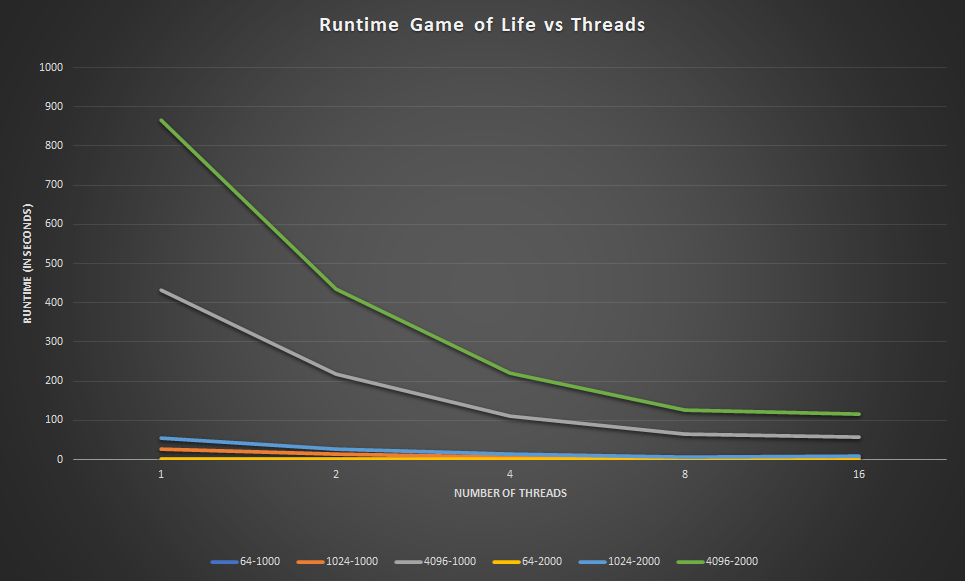
\includegraphics[width=\linewidth]{Figures/Runtimes.png}
    \caption{
        Runtime of Conway's Game of Life with no of threads $t \in \{1,2,4,8,16\}$
        dimensions $d \in \{64,1024,4096\}$ and timesteps $s \in \{1000,2000\}$.
    }
    \label{fig:cglspeedup}
\end{figure}

We see that the improvement reduce drastically and slows down between $8$ and $16$
threads. This is due to parallel slowdown (\cite{enwiki:ppslowdown}).
